\documentclass[lualatex,aspectratio=169,t,13pt,dvipsnames]{beamer}


%% References or not
%\usepackage[
%backend=biber,
%style=numeric,
%citestyle=numeric,
%giveninits=true
%]{biblatex}

%\renewcommand*{\bibfont}{\footnotesize}
%\addbibresource{refs.bib}

\usepackage[
outer/numbering=counter,
inner/sponsor/cern=true,
inner/sponsor/bmbf=false,
inner/sponsor/jgu=false,
inner/sponsor/fsp=false
]{theme/beamerthemeshiva}

%% Control over title font
% \setbeamerfont{title}{size=\fontsize{30pt}{30pt}, series=\bfseries, family=\avenir}

\usepackage{emoji}
\usepackage{pgfplots}
\usepackage{siunitx}
\usepackage{standalone}
\usepackage{tikz}
\usetikzlibrary{calc,external,decorations,decorations.pathmorphing,intersections,arrows,backgrounds,positioning,arrows.meta,decorations.text,backgrounds,shapes.geometric,positioning,fit,3d,pgfplots.colormaps,intersections,tikzmark}
\tikzset{>={Triangle[angle=35:3pt 3]}}

\directlua{os.execute("mkdir -p _tikz")}
\directlua{os.execute("mkdir -p build.nosync/_tikz")}
\tikzexternalize[prefix=_tikz/]

\usepackage[
  outputdir=build.nosync,
  newfloat
]{minted} 
\setminted{
%   bgcolor=code-gray,
%   samepage=true,
  autogobble,
  fontsize=\scriptsize,
}

\usepackage{svg}

%% Use head from prompt input

% THIS FILE IS AUTOGENERATED! EDIT WITH CAUTION
\title{Example reconstruction\\ chain walkthrough}
\date[ACTS4NP Workshop @ Berkeley 2025]{2025-05-12}
\author[paul.gessinger@cern.ch]{Paul Gessinger}
\institute{CERN}



%% Or customize 

% \title{Example reconstruction chain walkthrough}
% \date{2025-05-12}
% \author{Paul Gessinger}
% \institute{CERN}

\begin{document}

\maketitle

\section{Introduction}

\begin{frame}{ACTS Development Setup}
  \begin{itemize}
    \item ACTS = A Common Tracking Software
    \item Two main options for development setup:
    \begin{itemize}
      \item Native spack (builds packages from source)
      \item Docker images (prebuilt dependencies)
    \end{itemize}
    \item Warning: Spack builds can be challenging due to:
    \begin{itemize}
      \item ROOT compatibility issues
      \item Compiler/OS/library incompatibilities
      \item Build recipes not always updated
    \end{itemize}
  \end{itemize}
\end{frame}

\section{Docker Setup}
\begin{frame}[fragile]{Docker Images}
  \begin{itemize}
    \item Available prebuilt images with all dependencies
    \item Choose an image appropriate for your architecture from \cc{ghcr.io/acts-project/spack-container}
    \begin{itemize}
      \item x86\_64: \cc{9.2.0\_linux-ubuntu24.04-x86\_64\_gcc-13.3.0}
      \item aarch64: \cc{9.2.0\_linux-ubuntu24.04-aarch64\_gcc-13.3.0} (applies to ARM Macs)
    \end{itemize}
    \item Pull image using Docker:\\
    \begin{minted}[fontsize=\large]{bash}
      docker pull ghcr.io/acts-project/spack-container:$IMAGE
    \end{minted}
  \end{itemize}
\end{frame}

\begin{frame}[fragile]{Setting Up Docker Environment}
  \begin{itemize}
    \item Mount working directory into container
    \item Basic workflow:
    \begin{itemize}
      \item Start a container with working directory mounted
      \item Clone ACTS repository
      \item Compile and run ACTS
    \end{itemize}
    \item Command to start container:
  \end{itemize}
  
  \begin{minted}[fontsize=\large]{bash}
    docker run --rm -it -v $WORK:/work -w /work $IMAGE
  \end{minted}
  
  \begin{itemize}
    \item \cc{-v \$WORK:/work}: Mounts host directory into container
    \item \cc{-w /work}: Sets working directory inside container
    \item \cc{--rm}: Deletes container when stopped
    \item \cc{-it}: Creates interactive terminal session
  \end{itemize}
\end{frame}

\section{Building ACTS}
\begin{frame}[fragile]{Cloning ACTS}
  \begin{itemize}
    \item Clone the repository (inside container for \cc{git-lfs} access)
  \end{itemize}
  
  \begin{minted}[fontsize=\large]{bash}
    git clone https://github.com/acts-project/acts.git --recursive
  \end{minted}
  
  \begin{itemize}
    \item \cc{--recursive} flag is important to get OpenDataDetector submodule
  \end{itemize}
\end{frame}

\begin{frame}[fragile]{Building ACTS}
  \begin{itemize}
    \item Use CMake with presets for configuration
    \item For this tutorial: building Examples framework and OpenDataDetector
  \end{itemize}
  
  \begin{minted}[fontsize=\large]{bash}
    cmake -S $SOURCE_DIR -B build -G Ninja --preset dev \
      -DACTS_BUILD_UNITTESTS=OFF \
      -DACTS_BUILD_INTEGRATIONTESTS=OFF \
      -DACTS_BUILD_EXAMPLES_PYTHIA8=ON \
      -DACTS_BUILD_EXAMPLES_GEANT4=ON
  \end{minted}
  
  \begin{itemize}
    \item \cc{\$SOURCE\_DIR} is your ACTS clone (e.g., \cc{/work/acts})
    \item To build the project:
  \end{itemize}
  
  \begin{minted}[fontsize=\large]{bash}
    cmake --build build
  \end{minted}
\end{frame}

\begin{frame}{Build Optimizations}
  \begin{successblock}{\emoji{light-bulb} TIP: Persist \cc{ccache} caches between container runs}
    \begin{itemize}
      \item Mount host directory: \cc{-v \$WORK:/ccache}
      \item Do this before first build to benefit
    \end{itemize}
  \end{successblock}
  \begin{warnblock}{\emoji{warning} ACTS build requires significant memory}
    \begin{itemize}
      \item ~2-3GB per CPU core
      \item For memory issues: Limit cores with \cc{cmake --build -- -j\$N}
      \item Or reconfigure VM resources on macOS
    \end{itemize}
  \end{warnblock}
\end{frame}

\section{Preparing to Run}
\begin{frame}[fragile,c]{Installing Geant4 Data Files}
  \begin{itemize}
    \item Required for Geant4 simulation
    \item Install with:
  \end{itemize}
  
  \begin{minted}[fontsize=\large]{bash}
    geant4-config --install-datasets
  \end{minted}
  
  \begin{successblock}{\emoji{light-bulb} TIP: Persist Geant4 data files between container runs}
  \begin{itemize}
      \item Mount host directory: \cc{-v \$WORK:/g4data}
  \end{itemize}
  \end{successblock}
\end{frame}

\begin{frame}[fragile,c]{Setting Up Runtime Environment}
  \begin{itemize}
    \item Load runtime environment before running examples
  \end{itemize}
  
  \begin{minted}[fontsize=\large]{console}
    $ source build/this_acts_withdeps.sh
    INFO:    Found OpenDataDetector and set it up
    INFO:    Acts Python 3.13 bindings setup complete.
  \end{minted}
  
  \begin{itemize}
    \item Sets environment variables for ACTS Examples framework
    \item Activates dependencies: ROOT, DD4hep, Geant4
  \end{itemize}
\end{frame}

\section{Running ODD Example}

\begin{frame}{OpenDataDetector}
  \centering
  \only<1>{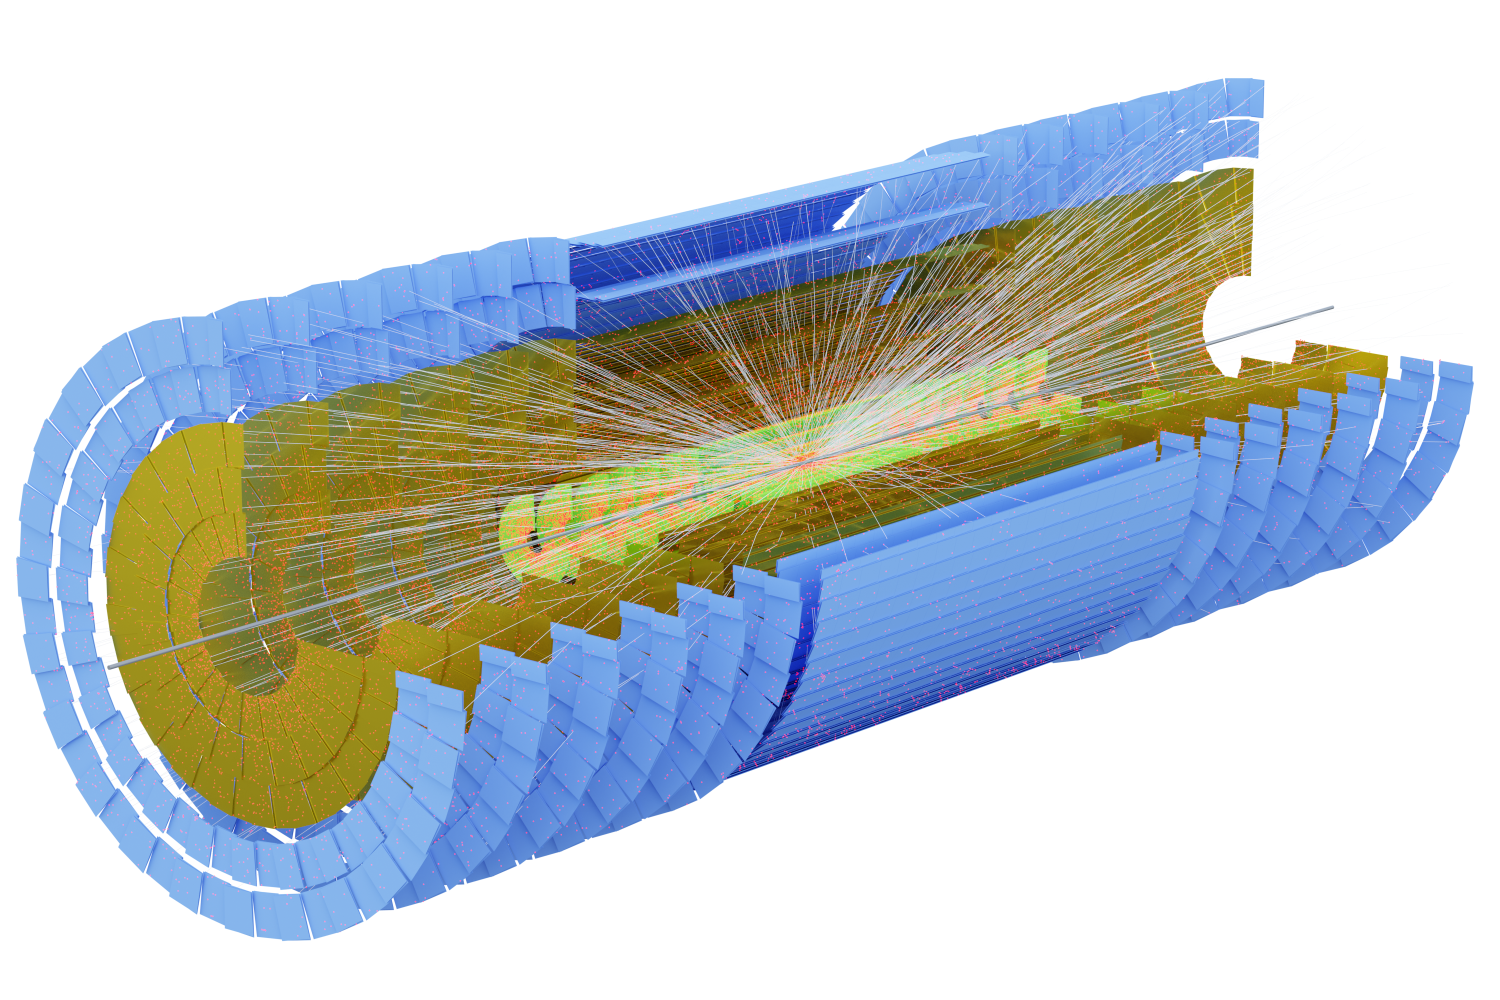
\includegraphics[width=0.7\textwidth]{figures/odd_glam.png}}
  \only<2>{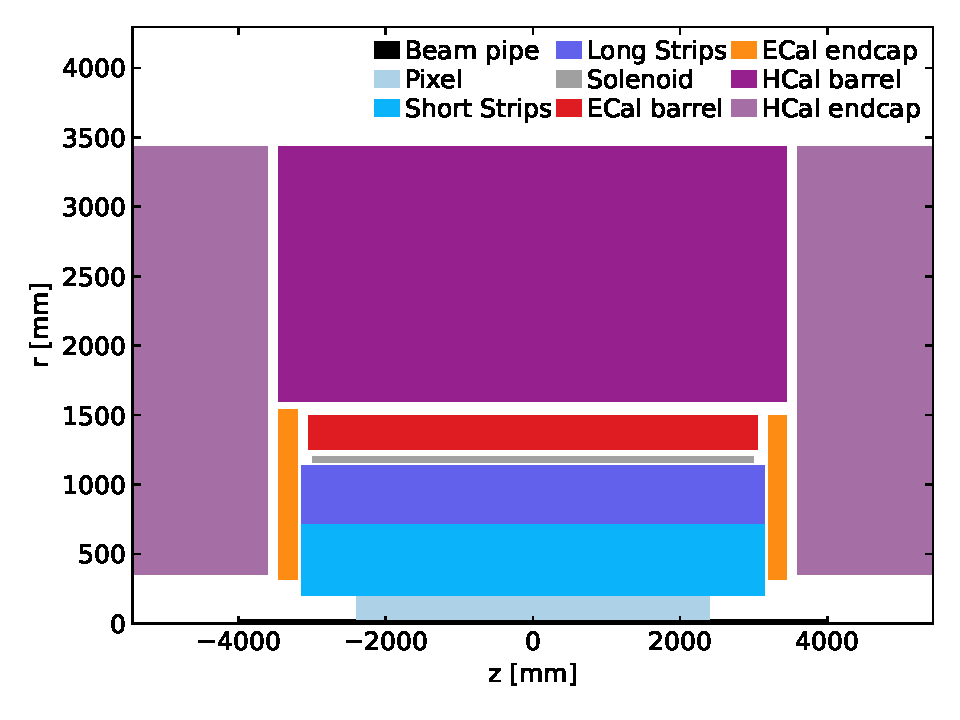
\includegraphics[width=0.7\textwidth]{figures/odd_layout.pdf}}
  \only<3>{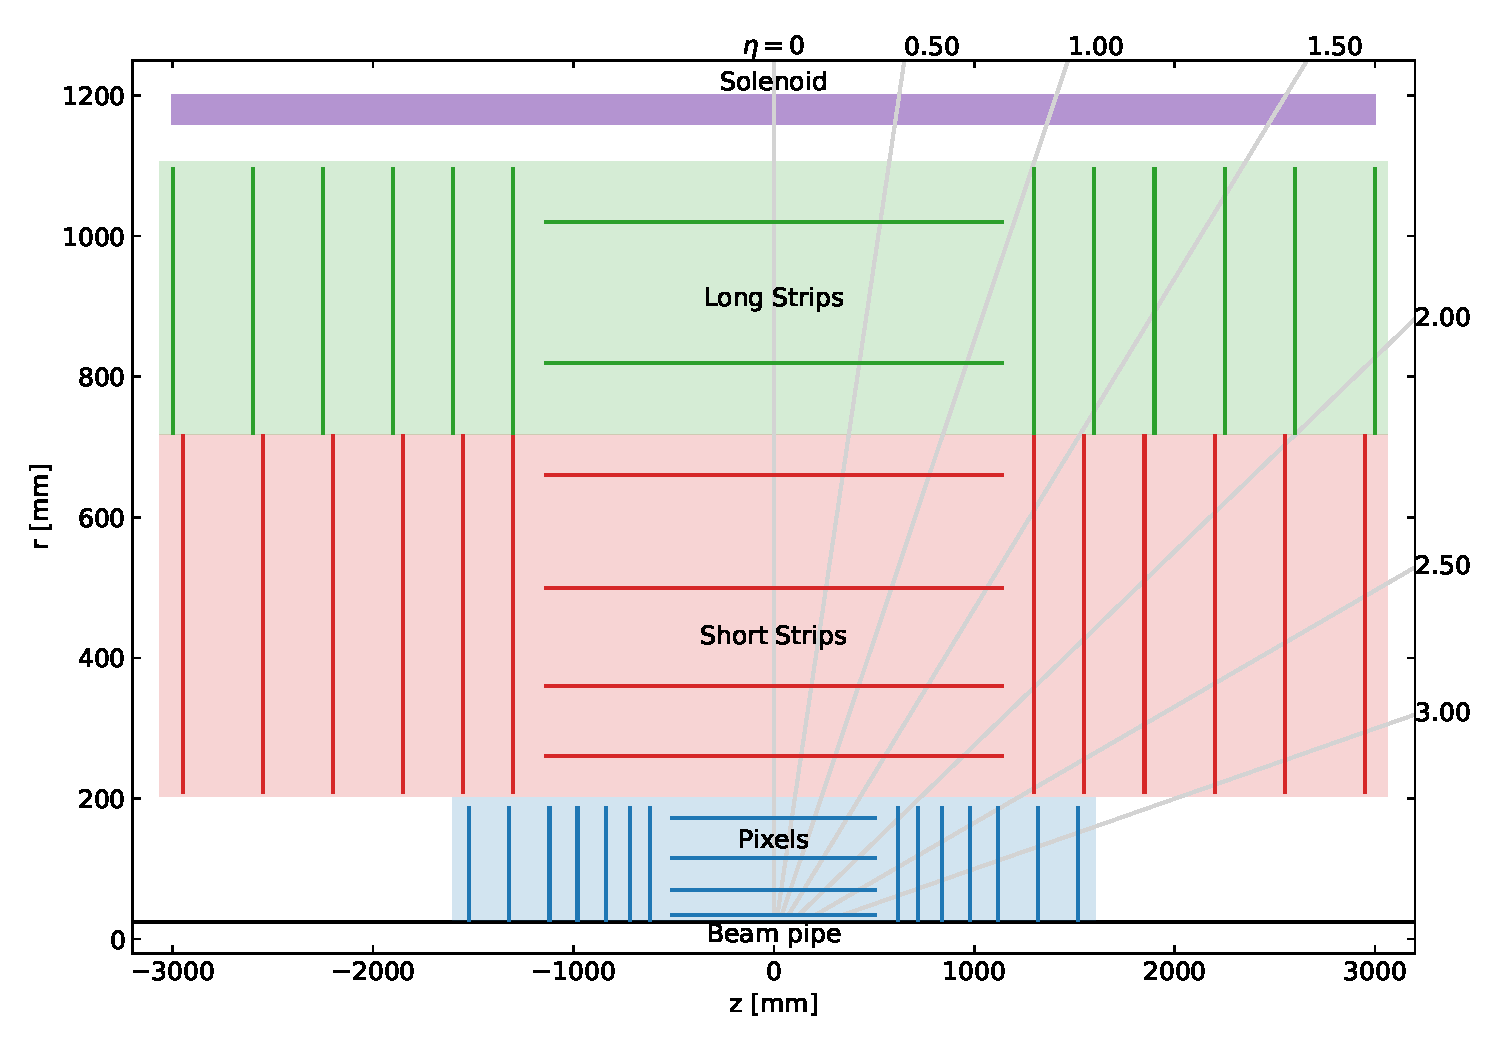
\includegraphics[width=0.7\textwidth]{figures/odd_tracker.pdf}}
\end{frame}

\begin{frame}[fragile,c]{ODD Workflow Example}
  \begin{minted}{console}
    $ Examples/Scripts/Python/full_chain_odd.py --help
    usage: full_chain_odd.py [-h] [--output OUTPUT] [--events EVENTS] [--skip SKIP] [--edm4hep EDM4HEP] 
                                  [--geant4] [--ttbar] [--ttbar-pu TTBAR_PU] 
                                  [--gun-particles GUN_PARTICLES] [--gun-multiplicity GUN_MULTIPLICITY]
                                  [--gun-eta-range GUN_ETA_RANGE GUN_ETA_RANGE] 
                                  [--gun-pt-range GUN_PT_RANGE GUN_PT_RANGE] [--digi-config DIGI_CONFIG]
                                  [--material-config MATERIAL_CONFIG] [--ambi-solver {greedy,scoring,ML}] 
                                  [--ambi-config AMBI_CONFIG] [--MLSeedFilter] [--reco | --no-reco]
                                  [--output-root | --no-output-root] [--output-csv | --no-output-csv] 
                                  [--output-obj | --no-output-obj]
  \end{minted}

  \begin{itemize}
    \item Default output directory: \cc{\$PWD/odd\_output}
  \end{itemize}
  \end{frame}

\begin{frame}[fragile,c]{ODD Workflow Example}


    \textbf{Example commands for different simulation scenarios:}
    \begin{itemize}
      \item Particle gun with fast simulation:
  
  \begin{minted}{bash}
    Examples/Scripts/Python/full_chain_odd.py -n10 --gun-multiplicity 10
  \end{minted}
  
    \item $t\bar{t}$ events with pile-up (fast simulation):
  
  \begin{minted}{bash}
    Examples/Scripts/Python/full_chain_odd.py -n10 --ttbar --ttbar-pu 10
  \end{minted}
  
    \item $t\bar{t}$ events with pile-up (Geant4 simulation):
  
  \begin{minted}{bash}
    Examples/Scripts/Python/full_chain_odd.py -n10 --ttbar --ttbar-pu 10 --geant4
  \end{minted}
  
  \end{itemize}

  \begin{successblock}{\emoji{light-bulb} TIP}
    \begin{itemize}
      \item Use \cc{--no-output-csv --no-output-obj} to speed up processing
      \item This will skip writing the CSV and ROOT files, which can take a while
    \end{itemize}
  \end{successblock}
\end{frame}

\section{ODD Script Components}
\begin{frame}{Core Concepts}
  \begin{itemize}
    \item Examples framework implements algorithm + event store processing loop
    \item Main components:
    \begin{itemize}
      \item \textbf{Sequencer}: Runs the event loop, configured with elements
      \item \textbf{Algorithms}: Main logic building blocks, call ACTS Core algorithms
      \item \textbf{Readers}: Read data from files or generate events
      \item \textbf{Writers}: Write data to files in various formats
    \end{itemize}
    \item Elements exchange information via entries in the event store
    \item Helper functions in \cc{acts.examples.reconstruction} and \cc{acts.examples.simulation} add sequence elements for specific tasks
  \end{itemize}
\end{frame}

\begin{frame}[fragile]{Detector Geometry Setup}
  \begin{minted}{python}
  # Figures out the source directory based on the location of this script
  geoDir = getOpenDataDetectorDirectory()

  # The material map is loaded from the common directory
  oddMaterialMap = (
      args.material_config
      if args.material_config
      else geoDir / "data/odd-material-maps.root"
  )

  # Configure digitization: defines sensitive detector elements and their measurements
  oddDigiConfig = (
      args.digi_config
      if args.digi_config
      else geoDir / "config/odd-digi-smearing-config.json"
  )
  \end{minted}
\end{frame}

\begin{frame}[fragile,c]{Digitization Process}
  \begin{itemize}
    \item Configured via JSON file (\cc{oddDigiConfig})
    \item Defines which detector elements are sensitive
    \item Determines what information is measured by each sensor
    \item Applies smearing to simulate detector resolution
    \item Example configuration entry:
  \end{itemize}
  
  \begin{minted}{json}
  {
    "volume": 16,
    "value": {
      "smearing": [
        { "index": 0, "stddev": 0.015, "type": "Gauss" },
        { "index": 1, "stddev": 0.015, "type": "Gauss" },
        { "index": 5, "stddev": 25, "type": "Gauss" }
      ]
    }
  }
  \end{minted}
\end{frame}



\begin{frame}[fragile]{Detector Geometry Setup (cont.)}
  \begin{minted}{python}
  oddSeedingSel = geoDir / "config/odd-seeding-config.json"
  oddMaterialDeco = acts.IMaterialDecorator.fromFile(oddMaterialMap)

  # This actually constructs and configures the geometry
  detector = getOpenDataDetector(odd_dir=geoDir, mdecorator=oddMaterialDeco)
  trackingGeometry = detector.trackingGeometry()
  decorators = detector.contextDecorators()

  # Configures a constant B field along the z-axis
  field = acts.ConstantBField(acts.Vector3(0.0, 0.0, 2.0 * u.T))
  # Configure a stable random number sequence
  rnd = acts.examples.RandomNumbers(seed=42)

  # Configuration of the sequencer
  s = acts.examples.Sequencer(
      events=args.events,
      skip=args.skip,
      numThreads=1 if args.geant4 else 1,
      outputDir=str(outputDir),
  )
  \end{minted}
\end{frame}

\begin{frame}[fragile]{Event Generation Options}

  \begin{columns}[T]
    \column{0.5\textwidth}
    \begin{itemize}
      \item Particle Gun (default):
      \begin{itemize}
        \item Configurable number of particles with specific distributions
        \item Properties: $p_T$, $\phi$, $\eta$ ranges can be set via command line
      \end{itemize}
      \uncover<2->{
      \item Pythia8 $t\bar{t}$ generation (with \cc{--ttbar})
      \begin{itemize}
        \item Generates full $t\bar{t}$ events
        \item Configurable pile-up events (with \cc{--ttbar-pu N})
      \end{itemize}
      }
      \uncover<3->{
      \item EDM4hep input option for existing events (with \cc{--edm4hep}) (\textbf{WIP})
      }
    \end{itemize}
    \column{0.5\textwidth}
    \vspace*{-2em}
    \begin{onlyenv}<1>
    \begin{minted}{python}
      addParticleGun(
          s,
          MomentumConfig(args.gun_pt_range[0] * u.GeV,
                         args.gun_pt_range[1] * u.GeV,
                         transverse=True),
          EtaConfig(args.gun_eta_range[0], 
                    args.gun_eta_range[1]),
          PhiConfig(0.0, 360.0 * u.degree),
          ParticleConfig(args.gun_particles, 
                         acts.PdgParticle.eMuon, 
                         randomizeCharge=True),
          vtxGen=acts.examples.GaussianVertexGenerator(
              mean=acts.Vector4(0, 0, 0, 0),
              stddev=acts.Vector4(
                  0.0125 * u.mm, 0.0125 * u.mm, 
                    55.5 * u.mm, 1.0 * u.ns
              ),
          ),
          multiplicity=args.gun_multiplicity,
          rnd=rnd,
      )
    \end{minted}
    \end{onlyenv}

    \begin{onlyenv}<2>
    \begin{minted}{python}
      addPythia8(
          s,
          hardProcess=["Top:qqbar2ttbar=on"],
          npileup=args.ttbar_pu,
          vtxGen=acts.examples.GaussianVertexGenerator(
              mean=acts.Vector4(0, 0, 0, 0),
              stddev=acts.Vector4(
                  0.0125 * u.mm, 0.0125 * u.mm, 
                  55.5 * u.mm, 5.0 * u.ns
              ),
          ),
          rnd=rnd,
          outputDirRoot=outputDir,
          outputDirCsv=outputDir,
      )

      addGenParticleSelection(
          s,
          ParticleSelectorConfig(
              rho=(0.0, 24 * u.mm), absZ=(0.0, 1.0 * u.m),
              eta=(-3.0, 3.0), pt=(150 * u.MeV, None),
          ),
      )
    \end{minted}
    \end{onlyenv}

    % \begin{onlyenv}<3>
    % \begin{minted}{python}
    %   edm4hepReader = EDM4hepSimReader(
    %     inputPath=str(args.edm4hep),
    %     inputSimHits=["PixelBarrelReadout", ...,
    %        "LongStripEndcapReadout"],
    %     outputParticlesGenerator="particles_generated",
    %     outputParticlesSimulation="particles_simulated",
    %     outputSimHits="simhits",
    %     graphvizOutput="graphviz",
    %     dd4hepDetector=detector,
    %     trackingGeometry=trackingGeometry,
    %     sortSimHitsInTime=True,
    %     level=acts.logging.INFO,
    %   )
    %   s.addReader(edm4hepReader)

    %   s.addWhiteboardAlias("particles", 
    %     edm4hepReader.config.outputParticlesGenerator)

    %   addGenParticleSelection(
    %       s,
    %       ParticleSelectorConfig(
    %           rho=(0.0, 24 * u.mm), absZ=(0.0, 1.0 * u.m),
    %           eta=(-3.0, 3.0), pt=(150 * u.MeV, None),
    %       ),
    %   )
    % \end{minted}
    % \end{onlyenv}

  \end{columns}
\end{frame}

\begin{frame}{Particle properties}
  \centering
  \resizebox{!}{\textheight-4em}{\includesvg{figures/particle_eta.svg}}
\end{frame}

\begin{frame}{Particle properties}
  \centering
  \resizebox{!}{\textheight-4em}{\includesvg{figures/particles_pt.svg}}
\end{frame}


\begin{frame}{Vertex properties}
  \centering
  \resizebox{0.5\textwidth}{!}{\includesvg{figures/vertices_vz.svg}}%
  \resizebox{0.5\textwidth}{!}{\includesvg{figures/vertices_vy.svg}}
\end{frame}


\begin{frame}[fragile]{Simulation Options}

  \begin{columns}[T]
    \column{0.5\textwidth}
    \begin{itemize}
      \item Two simulation backends:
      \begin{itemize}
        \uncover<1->{ \item \textbf{Geant4}: Full detector simulation \\
              (with \cc{--geant4})}
        \uncover<2->{\item \textbf{FATRAS}: ACTS Fast Simulation (default)}
      \end{itemize}
      \uncover<3->{
      \item Both produce:
      \begin{itemize}
        \item Simulated particles (\cc{particles\_simulated.root})
        \item Hits (\cc{hits.root})
      \end{itemize}
      }
    \end{itemize}

    \column{0.5\textwidth}
    \vspace*{-2em}

    \begin{onlyenv}<1>
    \begin{minted}{python}
      addGeant4(
            s,
            detector,
            trackingGeometry,
            field,
            outputDirRoot=outputDir,
            outputDirCsv=outputDir,
            outputDirObj=outputDir,
            rnd=rnd,
            killVolume=\
              trackingGeometry.highestTrackingVolume,
            killAfterTime=25 * u.ns,
        )
    \end{minted}
    \end{onlyenv}

    \begin{onlyenv}<2>
    \begin{minted}{python}
        addFatras(
            s,
            trackingGeometry,
            field,
            enableInteractions=True,
            outputDirRoot=outputDir,
            outputDirCsv=outputDir,
            outputDirObj=outputDir,
            rnd=rnd,
        )
    \end{minted}
    \end{onlyenv}

  \end{columns}
\end{frame}

\begin{frame}{Simulated particle properties}
  \centering
  \resizebox{0.5\textwidth}{!}{\includesvg{figures/sim_ptcl_pt.svg}}%
  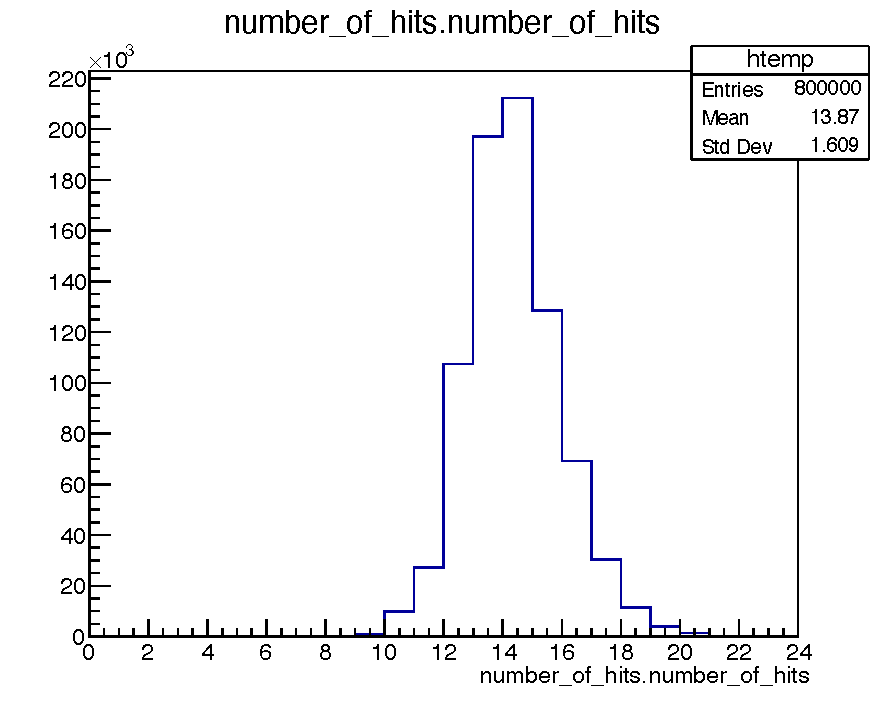
\includegraphics[width=0.5\textwidth]{figures/sim_ptcl_nhits.pdf}
\end{frame}

\begin{frame}{Simulated particle properties (cont.)}
  \centering
  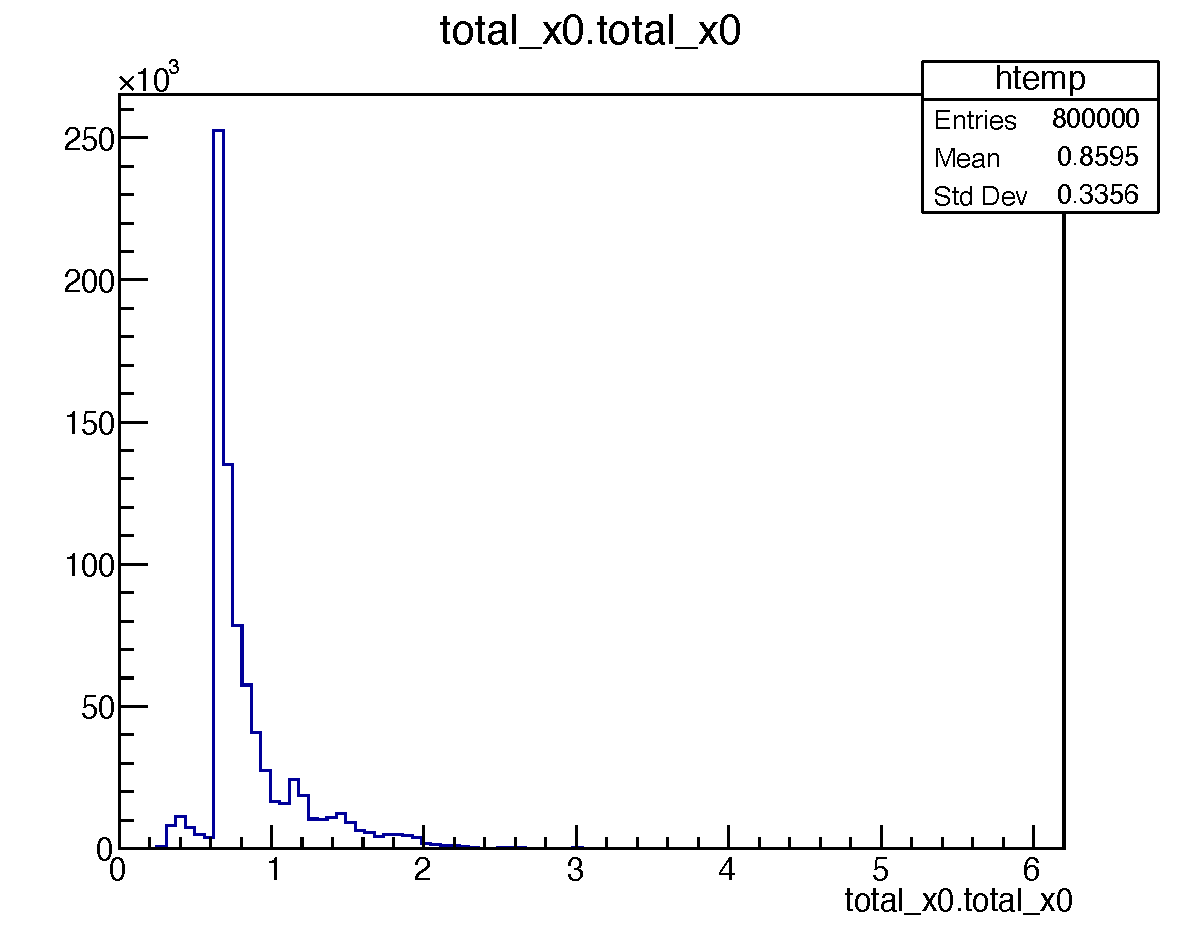
\includegraphics[width=0.5\textwidth]{figures/sim_ptcl_x0.pdf}%
  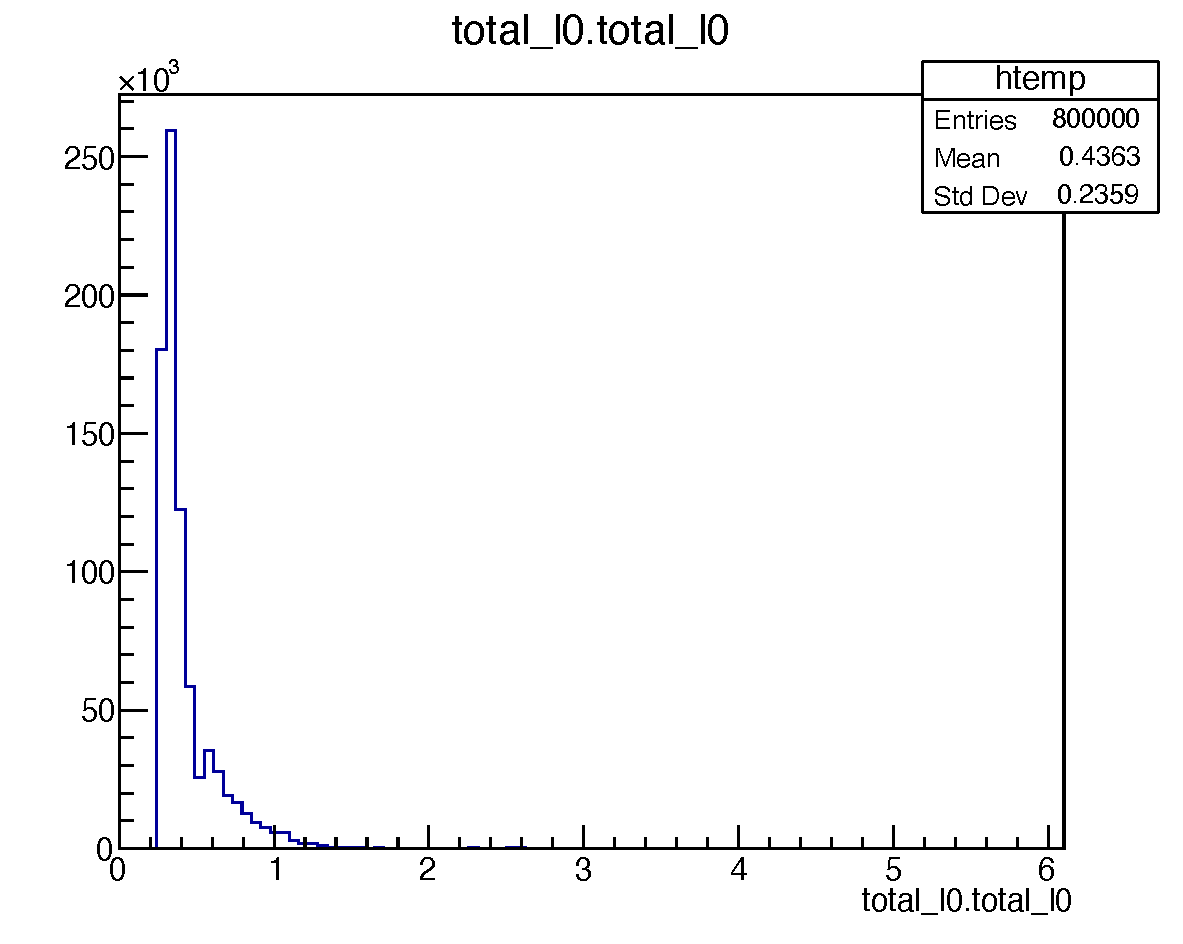
\includegraphics[width=0.5\textwidth]{figures/sim_ptcl_l0.pdf}
\end{frame}

\begin{frame}{Simulated particle properties (cont.)}
  \centering
  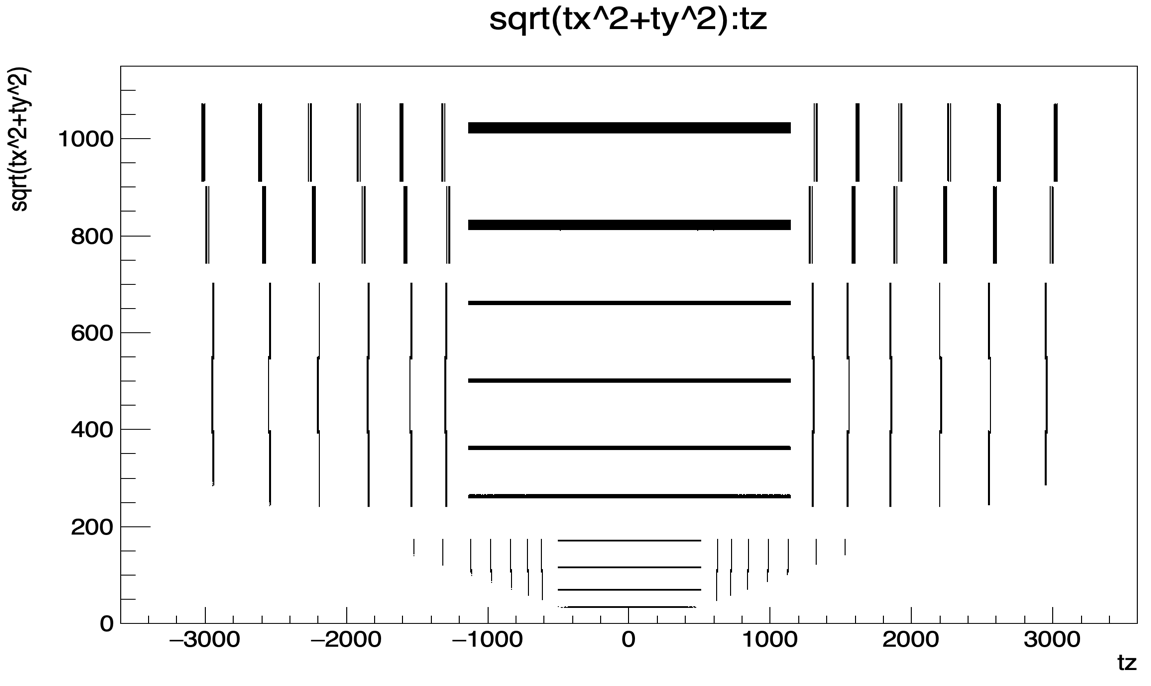
\includegraphics[height=\textheight-3em]{figures/hits_rz.png}%
\end{frame}

\begin{frame}[fragile,c]{Digitization}
  \begin{minted}{python}
    addDigitization(
      s,
      trackingGeometry,
      field,
      digiConfigFile=oddDigiConfig,
      outputDirRoot=outputDir if args.output_root else None,
      outputDirCsv=outputDir if args.output_csv else None,
      rnd=rnd,
    )
  \end{minted}

  \begin{itemize}
    \item Configures digitization process using JSON config file
    \begin{itemize}
      \item Adds DigitizationAlgorithm from Examples framework
      \item Handles both digitization and clustering if needed
      \item For smearing digitization, clustering is skipped
    \end{itemize}
    \item With configuration from before: Converts simulated hits to detector measurements via smearing
  \end{itemize}
\end{frame}

\begin{frame}{Cluster properties}
  \centering
  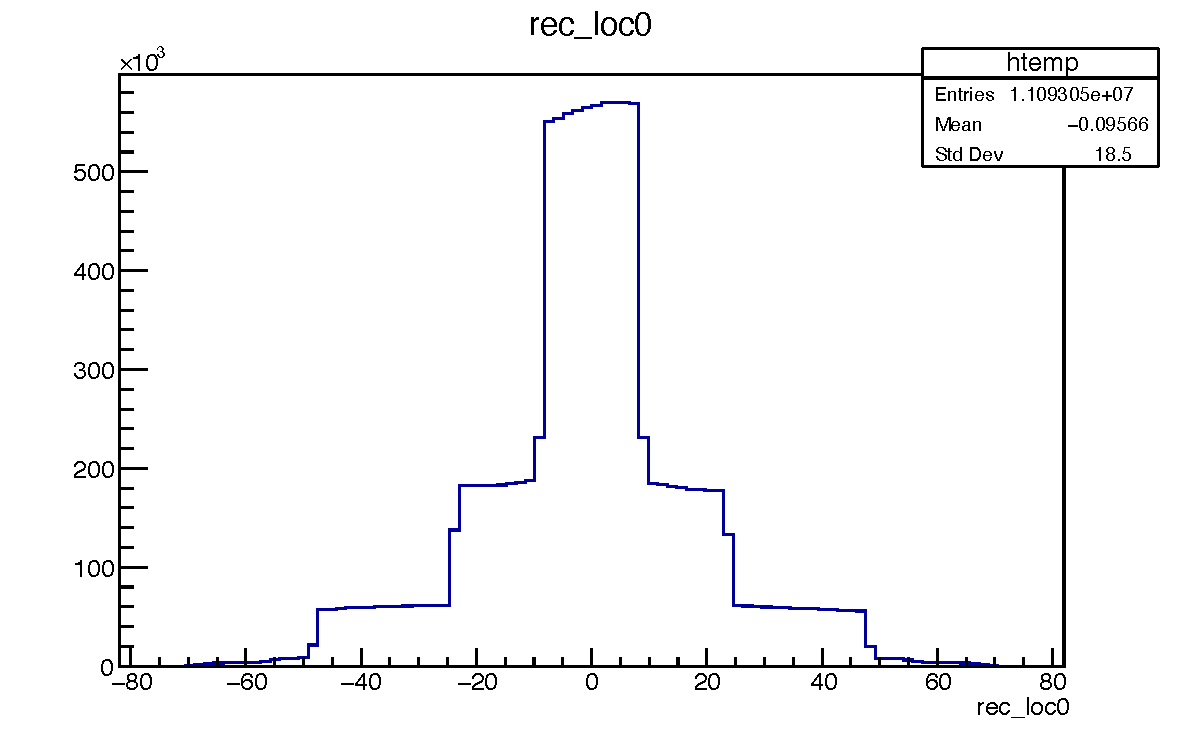
\includegraphics[width=0.5\textwidth]{figures/cluster_loc0.pdf}%
  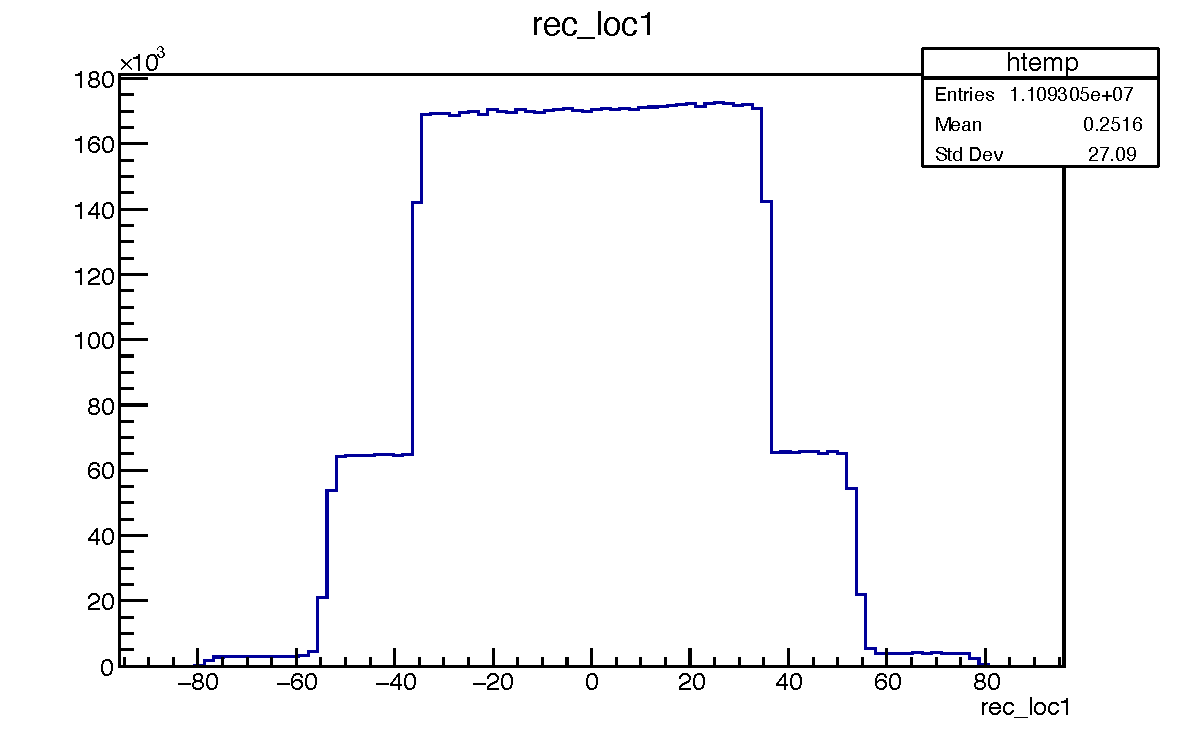
\includegraphics[width=0.5\textwidth]{figures/cluster_loc1.pdf}
  \begin{itemize}
    \item Shoulders \to{} sensor sizes
    \item Cluster uncertainties and pull distributions available
    \begin{itemize}
      \item For Gaussian smearing: expect normal pull distribution
      \item Uncertainties match smearing configuration in smeared digitization mode
    \end{itemize}
  \end{itemize}
\end{frame}


\begin{frame}[fragile,c]{Particle Selection}
  \begin{minted}{python}
addDigiParticleSelection(
    s,
    ParticleSelectorConfig(
        pt=(1.0 * u.GeV, None),
        eta=(-3.0, 3.0),
        measurements=(9, None),
        removeNeutral=True,
    ),
)
  \end{minted}
  
  \begin{itemize}
    \item Selection criteria:
    \begin{itemize}
      \item Minimum $p_T$ of 1.0 GeV
      \item $\eta$ range of $\pm$3.0
      \item At least 9 measurements
      \item Neutral particles removed
    \end{itemize}
  \end{itemize}
\end{frame}

\section{Reconstruction}

\begin{frame}[fragile]{Track Seeding}
  \begin{columns}
    \begin{column}{0.5\textwidth}
      \begin{itemize}
        \item First step in reconstruction pipeline
        \item Available seeding strategies:
        \begin{itemize}
          \item Full triplet seeding (Default)
          \item Truth smeared
          \item Truth estimated
          \item Orthogonal range seeding
          \item Others
        \end{itemize}
      \item Outputs:
      \begin{itemize}
        \item \cc{estimatedparams.root}: Track parameter information from seeds
        \item \cc{performance\_seeding.root}: Seeding efficiency information
      \end{itemize}
      \end{itemize}
    \end{column}
    \begin{column}{0.5\textwidth}
      \begin{minted}{python}
      addSeeding(
          s,
          trackingGeometry,
          field,
          initialSigmas=[
              1 * u.mm, 1 * u.mm, 
              1 * u.degree, 1 * u.degree,
              0.1 * u.e / u.GeV, 1 * u.ns,
          ],
          initialSigmaPtRel=0.1,
          initialVarInflation=[1.0] * 6,
          geoSelectionConfigFile=oddSeedingSel,
          outputDirRoot=outputDir,
          outputDirCsv=outputDir,
      )
      \end{minted}
    \end{column}
  \end{columns}
\end{frame}

\begin{frame}{Seed properties}
  \centering
  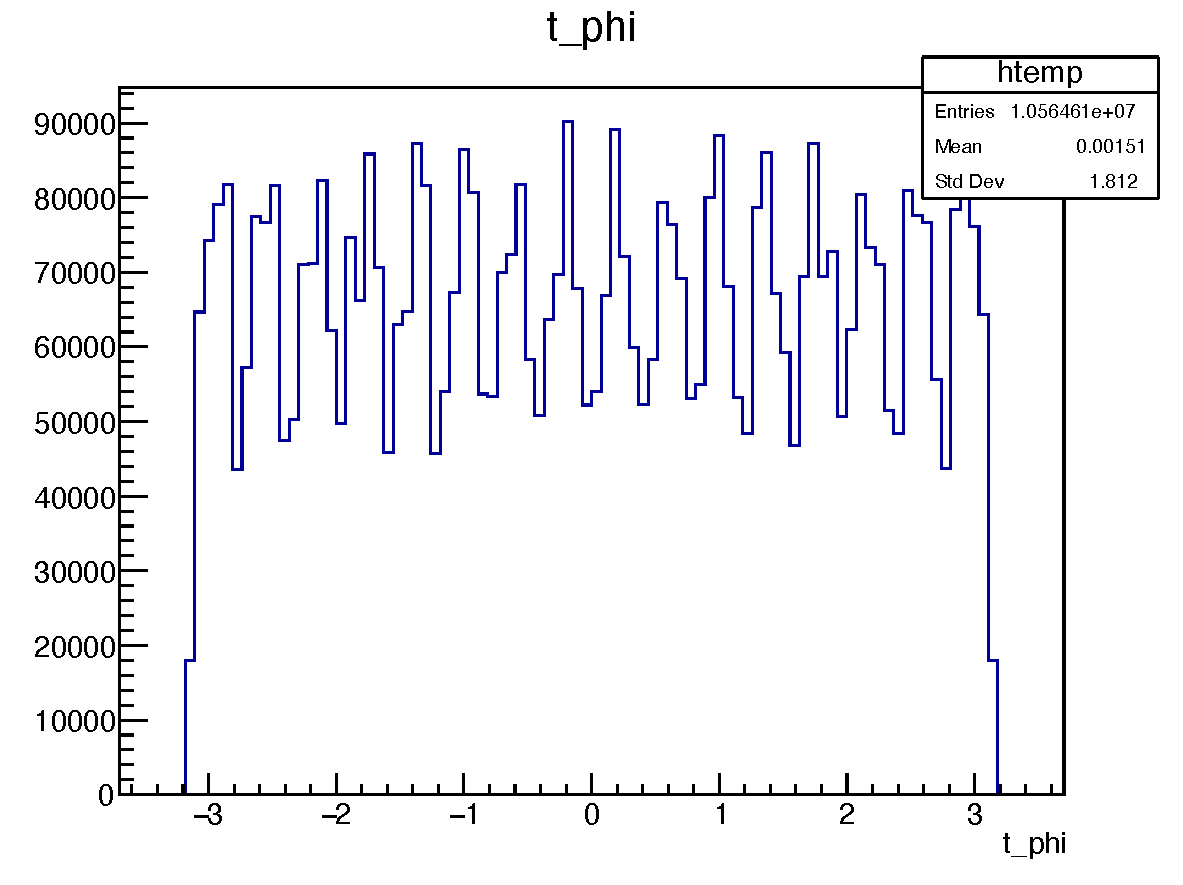
\includegraphics[width=0.5\textwidth]{figures/seed_phi.pdf}%
  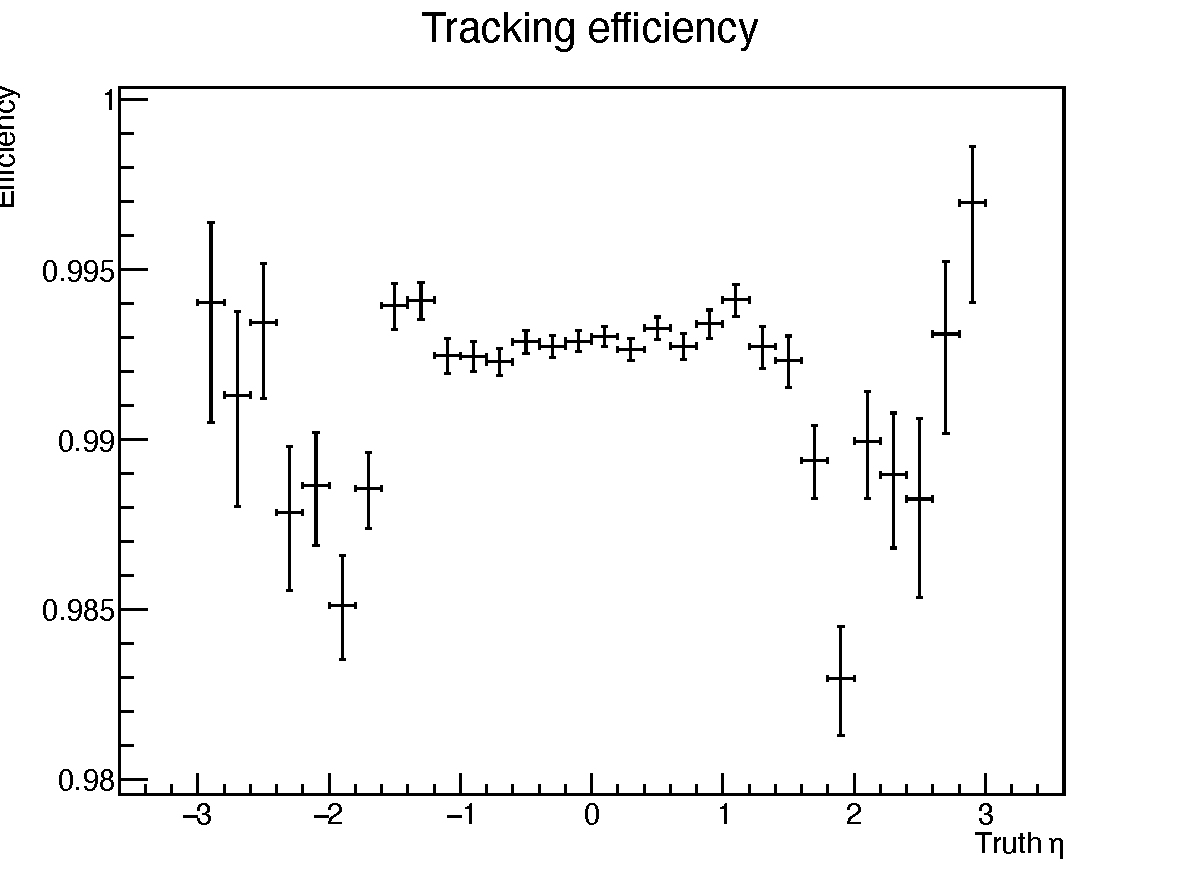
\includegraphics[width=0.5\textwidth]{figures/seed_eff_eta.pdf}
\end{frame}

\begin{frame}{Combinatorial Kalman Filter (CKF)}
  \begin{itemize}
    \item Main algorithm for track finding in ACTS
    \item Performance is highly sensitive to configuration
    \item Parameters to control:
    \begin{itemize}
      \item Track selection criteria
      \item $\chi^2$ cut-offs
      \item Volume constraints
      \item Measurement handling
      \item Seed handling
    \end{itemize}
  \end{itemize}
\end{frame}

\begin{frame}[fragile]{CKF Configuration}
  \begin{minted}{python}
addCKFTracks(
    s,
    trackingGeometry,
    field,
    TrackSelectorConfig(
        pt=(1.0 * u.GeV if args.ttbar else 0.0, None), absEta=(None, 3.0),
        loc0=(-4.0 * u.mm, 4.0 * u.mm), nMeasurementsMin=7, maxHoles=2, maxOutliers=2,
    ),
    CkfConfig(
        chi2CutOffMeasurement=15.0,  # Valid measurement threshold
        chi2CutOffOutlier=25.0,      # Outlier threshold
        numMeasurementsCutOff=10,    # Max measurements to consider
        seedDeduplication=True,      # Use each seed once
        stayOnSeed=True,             # Force inclusion of seed measurements
        pixelVolumes=[16, 17, 18],   # Volume ID mapping
        stripVolumes=[23, 24, 25],
        maxPixelHoles=1, maxStripHoles=2,
        constrainToVolumes=[...],    # Restrict to specific volumes
    ),
    outputDirRoot=outputDir, outputDirCsv=outputDir, writeCovMat=True,
)
  \end{minted}
\end{frame}

\begin{frame}{CKF outputs}
  \begin{itemize}
    \item Track finding performance stored in \texttt{performance\_finding\_ckf.root}
    \item Track properties and quality in \texttt{performance\_fitting\_ckf.root}
    \item Ambiguity resolution needed to handle shared clusters:
    \begin{itemize}
      \item Multiple tracks can share measurement clusters
      \item Goal: Unique cluster-to-track association
    \end{itemize}
    \item Three available strategies:
    \begin{itemize}
      \item Machine learning based (ONNX model)
      \item Score-based (quality and hit content)
      \item Greedy (iterative removal by shared hit fraction)
    \end{itemize}
  \end{itemize}
\end{frame}

\begin{frame}{CKF outputs (cont.)}
  \centering
  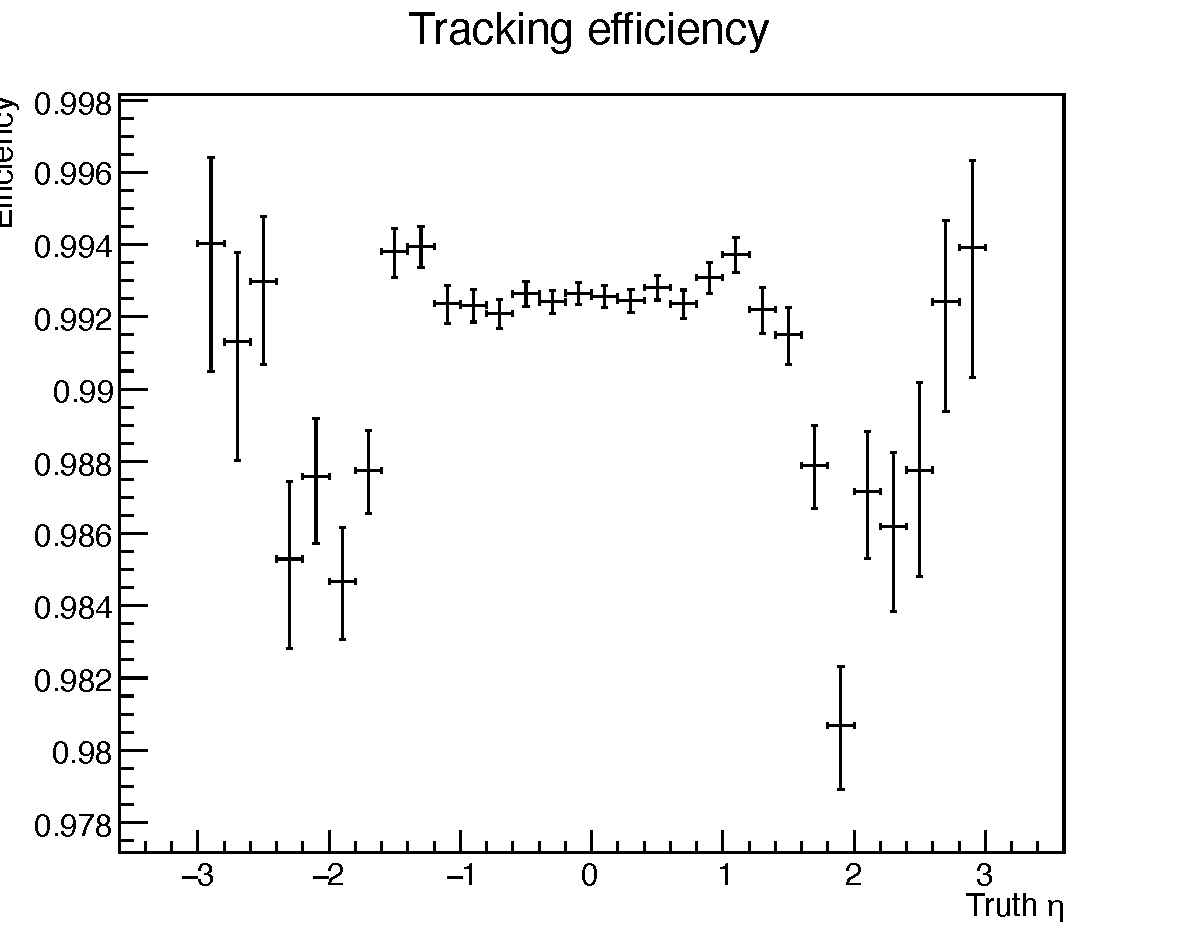
\includegraphics[width=0.5\textwidth]{figures/track_eff_eta.pdf}%
  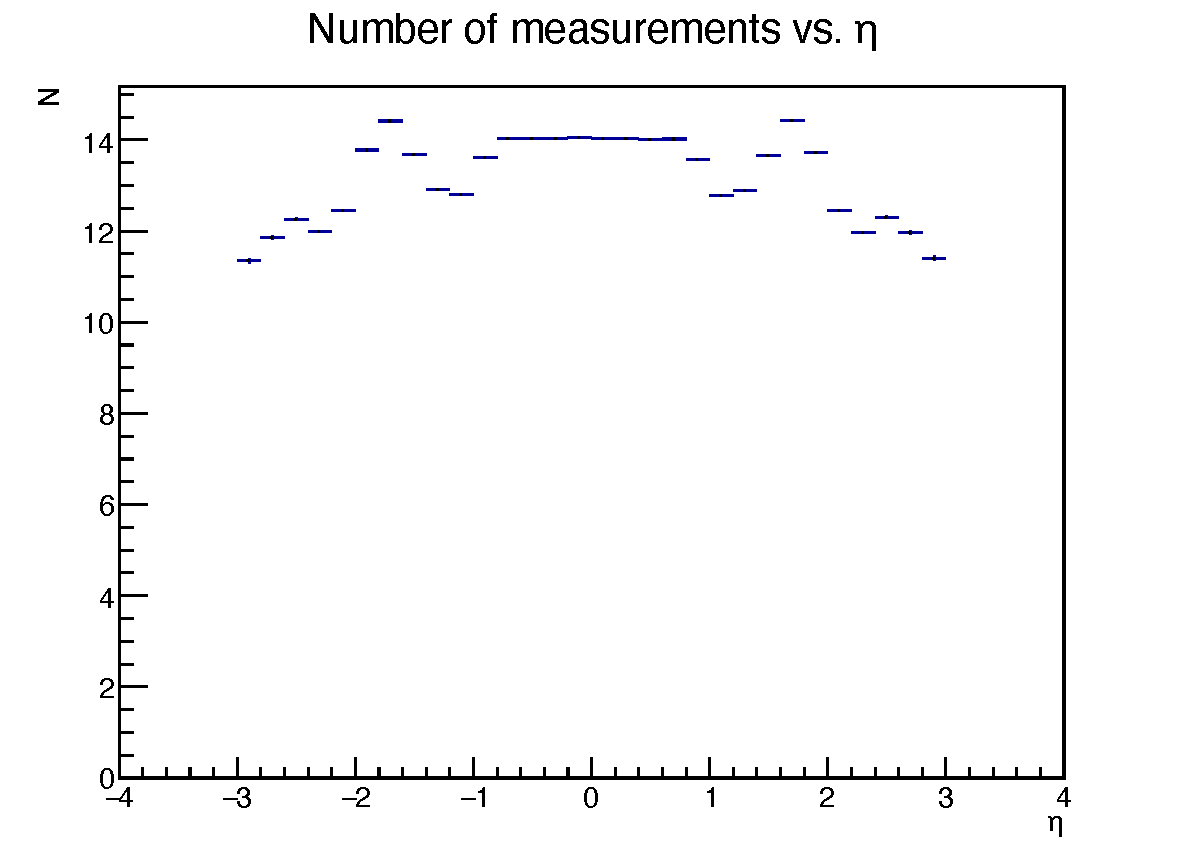
\includegraphics[width=0.5\textwidth]{figures/track_nmeas.pdf}
\end{frame}

\begin{frame}[fragile]{Ambiguity Resolution}
  \begin{minted}{python}
addAmbiguityResolution(
    s,
    AmbiguityResolutionConfig(
        maximumSharedHits=3,
        maximumIterations=1000000,
        nMeasurementsMin=7
    ),
    outputDirRoot=outputDir if args.output_root else None,
    outputDirCsv=outputDir if args.output_csv else None,
    writeCovMat=True,
)
  \end{minted}

  \begin{itemize}
    \item Same outputs produced for tracks after ambiguity resolution as for direct CKF outputs
    \item Performance metrics available in \texttt{performance\_finding\_ambi.root} and \texttt{performance\_fitting\_ambi.root}
  \end{itemize}
\end{frame}

\begin{frame}[fragile]{Final Processing and Output}
  \begin{itemize}
    \item Vertex fitting added as final step:
    \item Vertex outputs will be written to \cc{performance\_vertexing.root}
    \begin{minted}{python}
addVertexFitting(
    s,
    field,
    vertexFinder=VertexFinder.AMVF,
    outputDirRoot=outputDir if args.output_root else None,
)
    \end{minted}
    \item Run the full sequence:
    \begin{minted}[fontsize=\large]{python}
s.run()
    \end{minted}
    \item Output files include:
    \begin{itemize}
      \item Truth information: \cc{particles.root}, \cc{vertices.root}
      \item Simulation: \cc{particles\_simulated.root}, \cc{hits.root}
      \item Reconstruction: \cc{measurements.root}, \cc{performance\_*.root}
    \end{itemize}
  \end{itemize}
\end{frame}

\begin{frame}{Vertex properties}
  \centering
  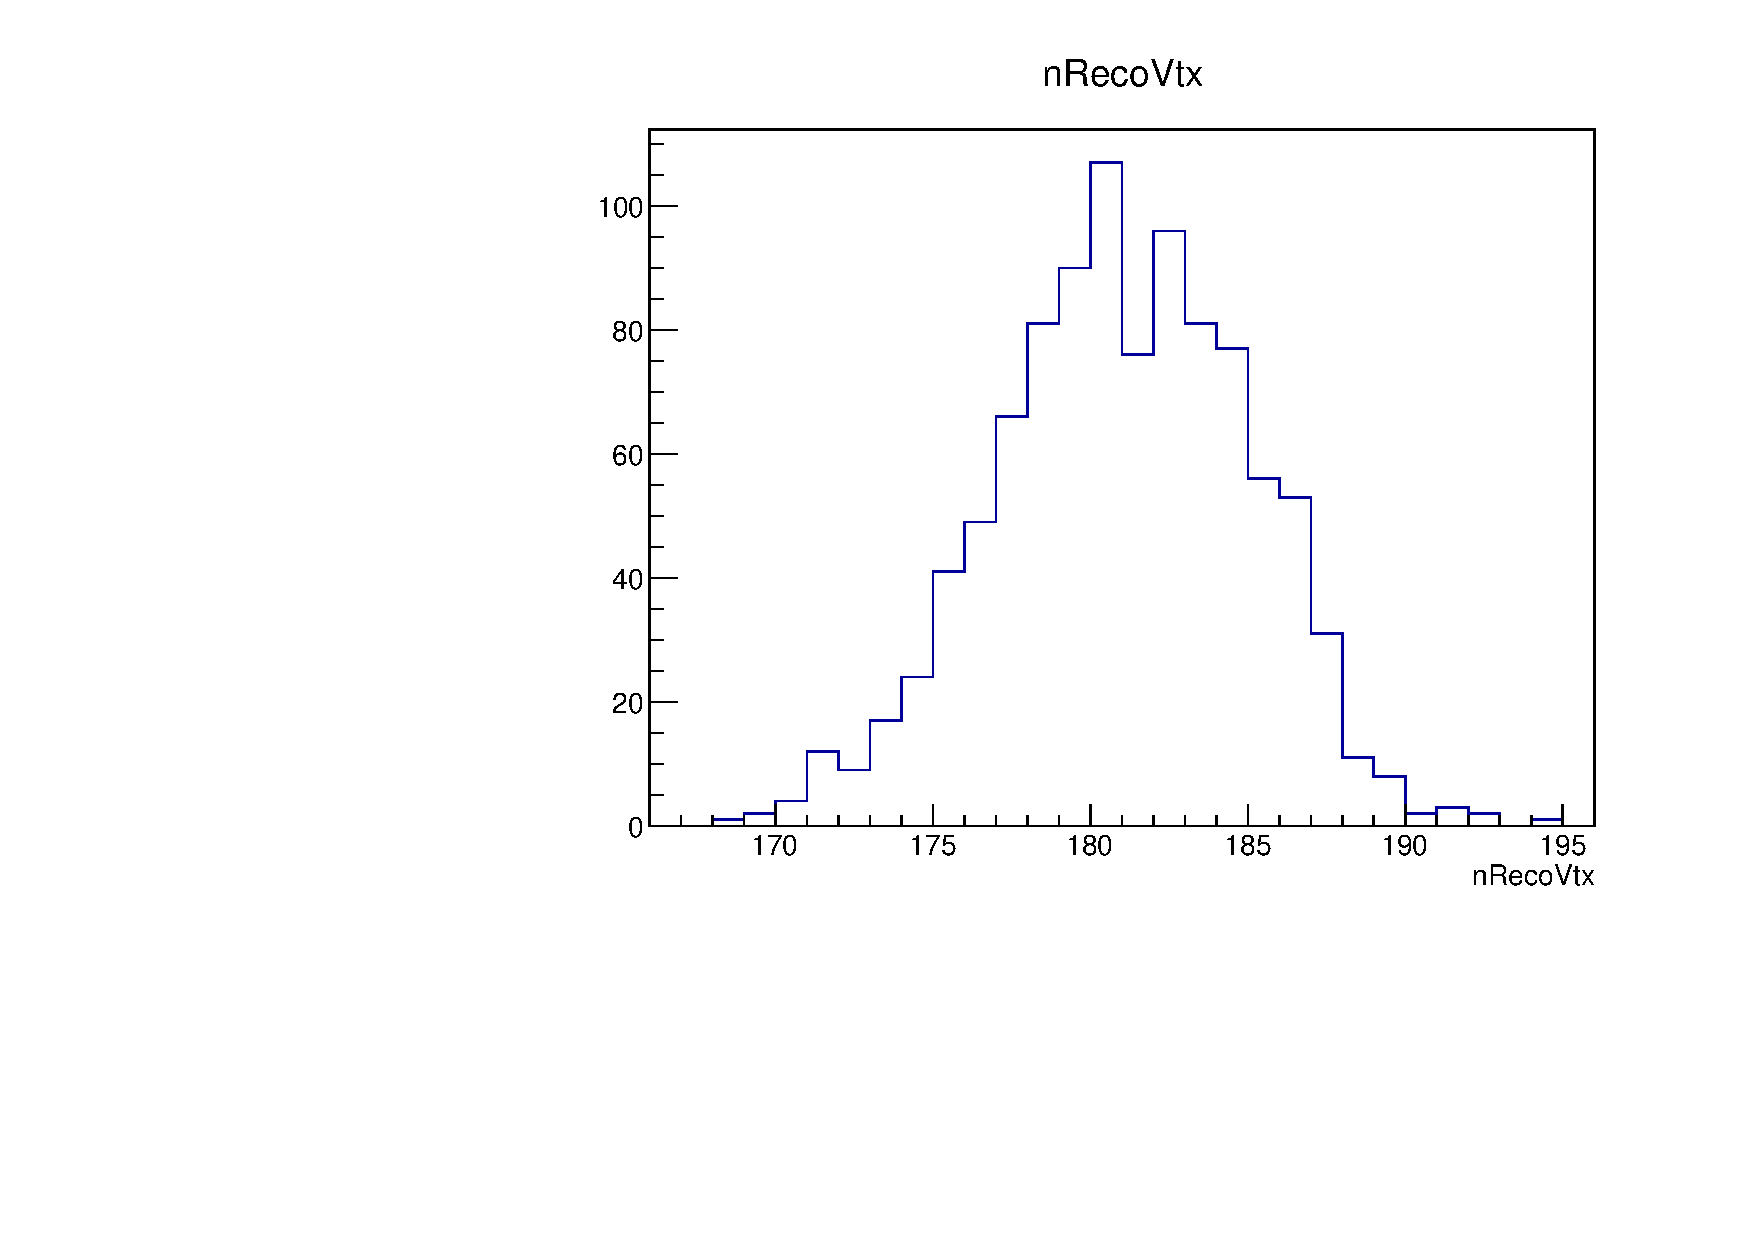
\includegraphics[width=0.5\textwidth]{figures/vertex_count.pdf}%
  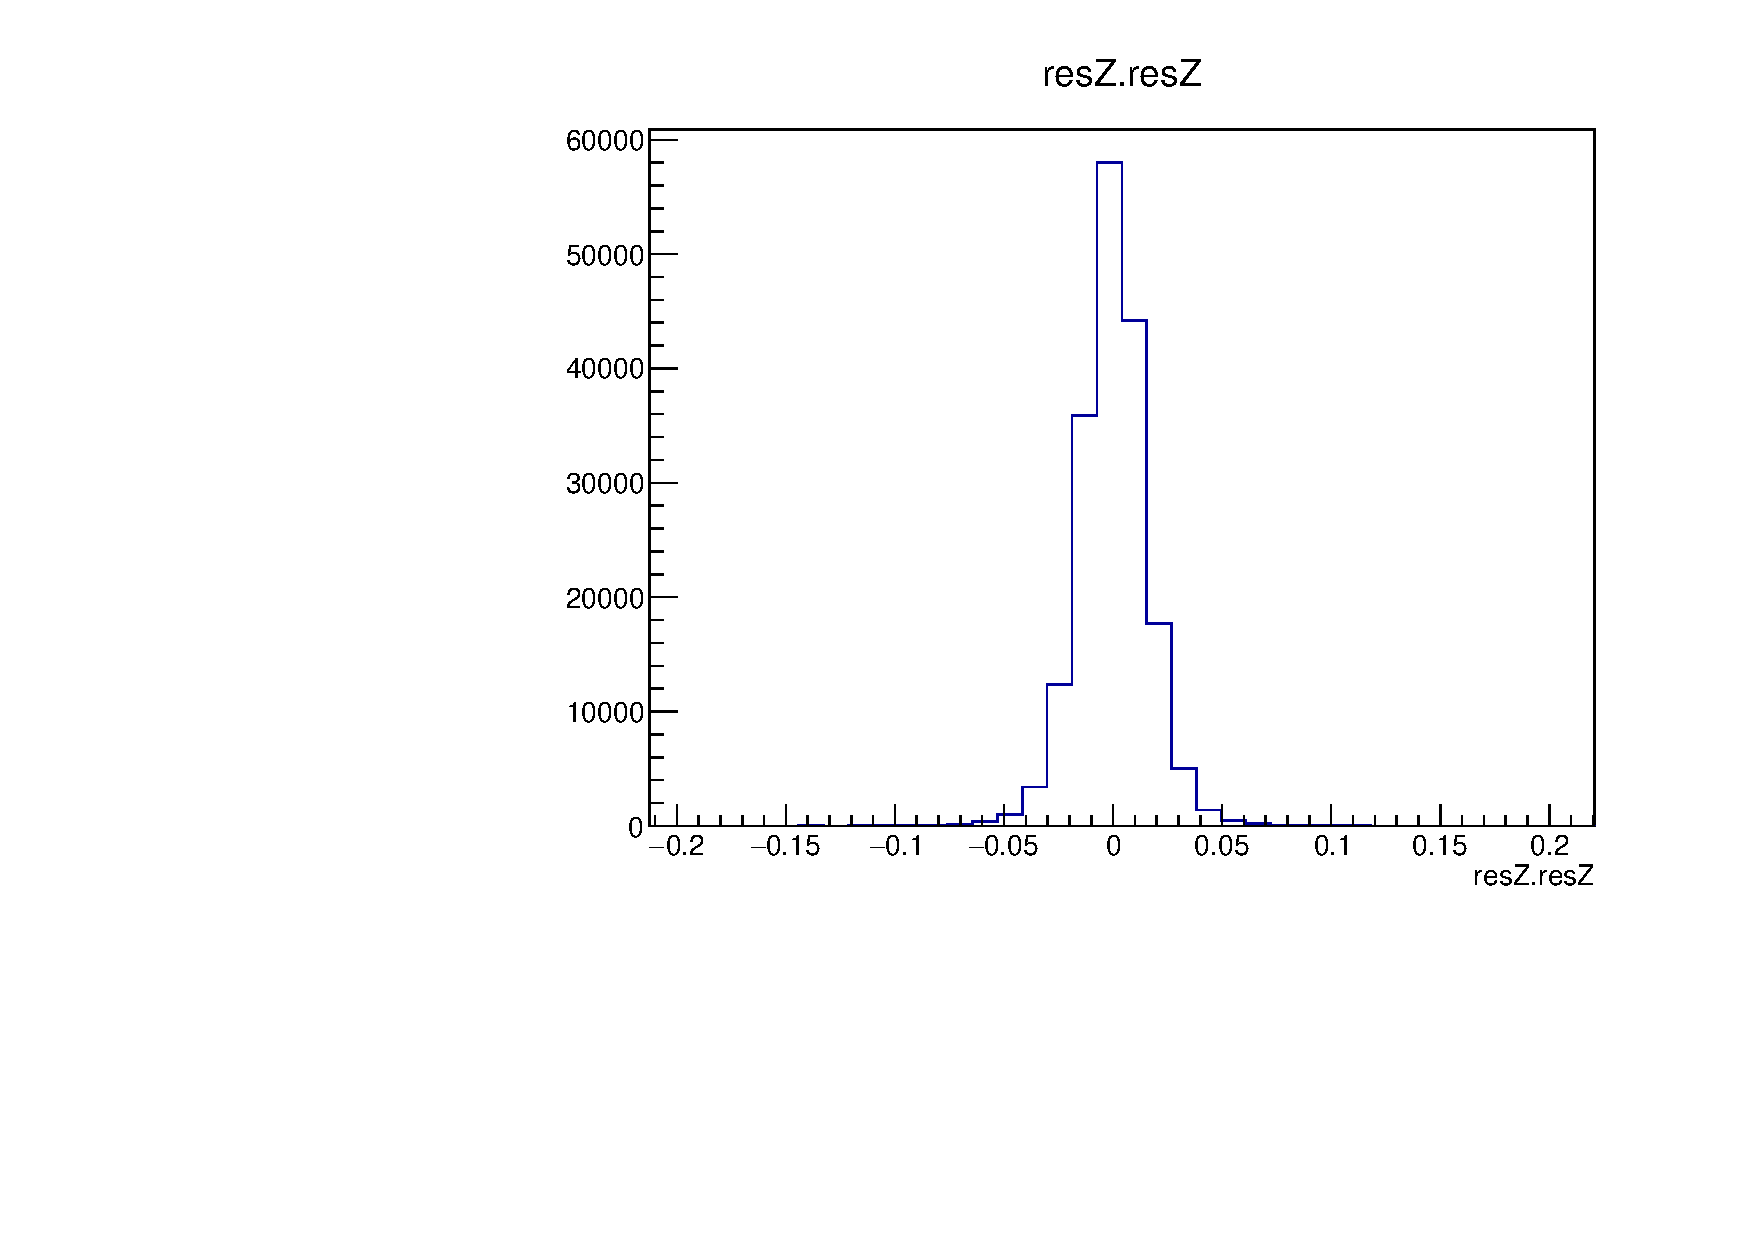
\includegraphics[width=0.5\textwidth]{figures/vertex_resz.pdf}
\end{frame}

% \section{Known Issues}
% \begin{frame}{Known Issues}
%   \begin{itemize}
%     \item Warning about parameter passing in GCC11 on aarch64
%     \begin{itemize}
%       \item ABI change in GCC11
%       \item Not actionable, only suppressible with \texttt{-Wno-psabi}
%       \item Add to CMake command: \texttt{-DCMAKE\_CXX\_FLAGS="-Wno-psabi"}
%     \end{itemize}
%   \end{itemize}
% \end{frame}

%% Uncomment if using references
%\begin{frame}[t,allowframebreaks]
  %\frametitle{References}
  %\printbibliography[heading=none]
%\end{frame}

\end{document}
